\section{Routes}

Die Routes zur Navigation durch den Admin-Client unterscheiden sich kaum von denen des normalen
Clients.\\
Aufgrund seines Zwecks benötigt diese Version des Clients keine Signup-Route, da die
Authentifikation mit ACP-Nutzern, die zuerst im \nameref{acp} erzeugt werden müssen, erfolgt.

Hierfür wird auf bekannte Weise eine HashMap mit den benötigten Routen erzeugt:

\begin{code}[H]
    \centering
    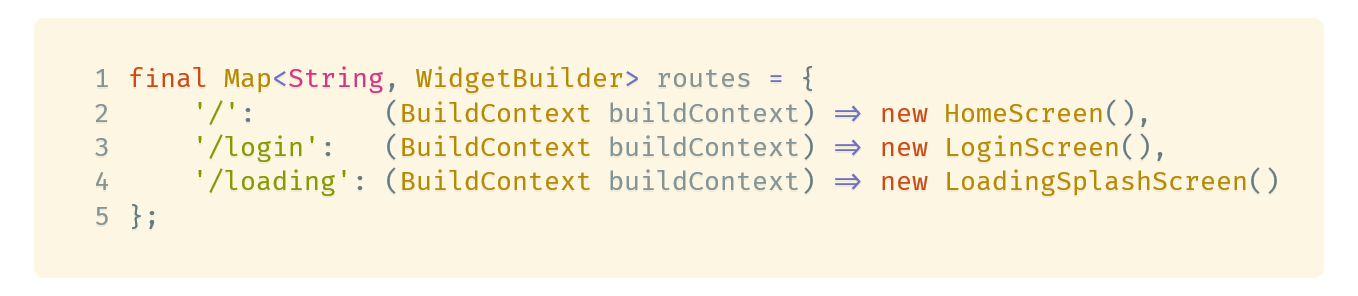
\includegraphics[width=1\textwidth]{images/Admin-Client/util/routes.png}
    \vspace{-25pt}
    \caption{Routes des Admin-Clients}
\end{code}